\documentclass[tikz,dvisvgm,border=0pt]{standalone}
% Shared look for every Tokimeki figure.
\usepackage[T1]{fontenc}
\usepackage{lmodern}
\usetikzlibrary{arrows.meta,calc,backgrounds,patterns}
\renewcommand{\familydefault}{\sfdefault}

\definecolor{ink}{HTML}{1F2D33}
\definecolor{muted}{HTML}{7A8A8C}
\definecolor{rule}{HTML}{A7B6B8}
\definecolor{diskfill}{HTML}{EEF1F0}
\definecolor{diskline}{HTML}{8FA3A5}
\definecolor{runfill}{HTML}{E3F2EC}
\definecolor{runline}{HTML}{3E8C70}
\definecolor{userfill}{HTML}{FFF1E0}
\definecolor{userline}{HTML}{C9843E}
\definecolor{orangefill}{HTML}{FCDDBA}
\definecolor{orangeline}{HTML}{D27F2F}
\definecolor{bluefill}{HTML}{D6E4F5}
\definecolor{blueline}{HTML}{4F7FB3}
\definecolor{redline}{HTML}{C0453A}
\definecolor{purplefill}{HTML}{E7DDF3}
\definecolor{purpleline}{HTML}{8462B3}

\tikzset{
  every node/.style={text=ink, font=\small},
  fig/.style={show background rectangle, background rectangle/.style={fill=white}, inner frame sep=12pt},
  % places
  disk/.style={draw=diskline, line width=0.9pt, fill=diskfill},
  runner/.style={draw=runline, line width=1pt, fill=runfill},
  user/.style={draw=userline, line width=1pt, fill=userfill},
  title/.style={font=\bfseries\small, anchor=north west},
  where/.style={font=\footnotesize, text=muted, anchor=north west},
  % things
  card/.style={draw=rule, line width=0.8pt, fill=white,
               minimum width=1.9cm, minimum height=0.62cm, inner sep=2pt, font=\ttfamily\scriptsize},
  groupA/.style={card, draw=orangeline, fill=orangefill},
  groupB/.style={card, draw=blueline, fill=bluefill},
  groupC/.style={card, draw=purpleline, fill=purplefill},
  slot/.style={draw=runline!55, line width=0.8pt, dash pattern=on 2.5pt off 1.8pt, fill=white,
               minimum width=2.1cm, minimum height=0.8cm},
  cmd/.style={fill=ink, text=white, font=\ttfamily\scriptsize, inner sep=4pt, anchor=south west},
  % arrows: solid = write a file, dashed = read a file
  write/.style={-{Stealth[length=6.5pt,width=5.5pt]}, line width=1.2pt},
  read/.style={-{Stealth[length=6.5pt,width=5.5pt]}, line width=1.1pt, dash pattern=on 4pt off 2.5pt},
  lbl/.style={font=\footnotesize, fill=white, inner sep=1.5pt},
  num/.style={circle, fill=ink, text=white, font=\bfseries\scriptsize, inner sep=1pt, minimum size=12pt},
}

% \diskslab{x0}{y0}{x1}{y1}  -- the shared directory every node mounts
\newcommand{\diskslab}[4]{%
  \draw[disk] (#1,#2) rectangle (#3,#4);
  \node[font=\bfseries\footnotesize, text=diskline, anchor=south east] at (#3-0.15,#2+0.08)
    {shared filesystem};
}

% \machine{x0}{y0}{x1}{y1}{label} -- a physical node: white box with a dark header bar
\newcommand{\machine}[5]{%
  \draw[ink, line width=1pt, fill=white] (#1,#2) rectangle (#3,#4);
  \fill[ink] (#1,#4-0.5) rectangle (#3,#4);
  \fill[ink] (#1,#4-0.5) rectangle (#3,#4-0.3);
  \node[font=\bfseries\footnotesize, text=white, anchor=west] at (#1+0.15,#4-0.25) {#5};
}
% \proc{x0}{y0}{x1}{y1}{label} -- the runner daemon running on a node
\newcommand{\proc}[5]{%
  \draw[runner] (#1,#2) rectangle (#3,#4);
  \node[font=\bfseries\scriptsize, text=runline, anchor=north west] at (#1+0.1,#4-0.05) {#5};
}
% \tray{x0}{y0}{x1}{y1}{label} -- a place on the shared filesystem
\newcommand{\tray}[5]{%
  \draw[draw=rule, fill=white] (#1,#2) rectangle (#3,#4);
  \node[font=\footnotesize, text=muted, anchor=north east] at (#3-0.08,#4-0.03) {#5};
}
\tikzset{
  script/.style={draw=ink, line width=0.8pt, fill=white, font=\ttfamily\scriptsize,
                 minimum width=1.7cm, minimum height=1.0cm, inner sep=2pt,
                 append after command={\pgfextra{\let\n\tikzlastnode}
                   (\n.north east) ++(-0.28,0) -- ++(0,-0.28) -- ++(0.28,0)}},
}

\begin{document}
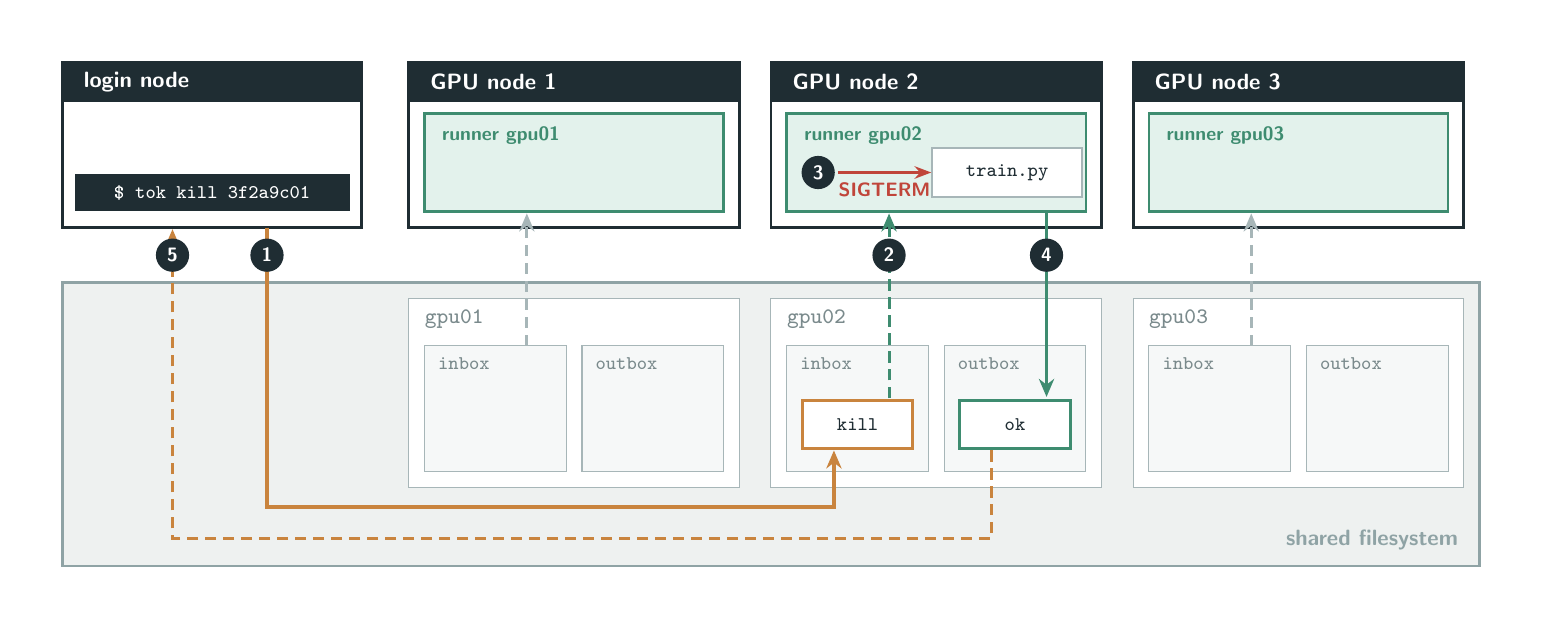
\begin{tikzpicture}[fig]
  \tikzset{box/.style={draw=rule, fill=diskfill!50},
           boxname/.style={font=\ttfamily\scriptsize, text=muted, anchor=north west},
           msg/.style={card, minimum width=1.4cm, line width=1.1pt}}

  % shared filesystem: one inbox and one outbox per runner
  \diskslab{0}{-0.6}{18.0}{3.0}
  \foreach \i/\x in {1/4.4, 2/9.0, 3/13.6} {
    \draw[draw=rule, fill=white] (\x,0.4) rectangle (\x+4.2,2.8);
    \node[boxname, font=\ttfamily\footnotesize] at (\x+0.08,2.78) {gpu0\i};
    \draw[box] (\x+0.2,0.6) rectangle (\x+2.0,2.2);
    \draw[box] (\x+2.2,0.6) rectangle (\x+4.0,2.2);
    \node[boxname] at (\x+0.25,2.17) {inbox};
    \node[boxname] at (\x+2.25,2.17) {outbox};
  }
  \node[msg, draw=userline] at (10.1,1.2) {kill};
  \node[msg, draw=runline] at (12.1,1.2) {ok};

  % login node
  \machine{0}{3.7}{3.8}{5.8}{login node}
  \node[cmd, minimum width=3.5cm, align=left] at (0.15,3.9) {\$ tok kill 3f2a9c01};

  % GPU nodes, each running a runner
  \foreach \i/\x in {1/4.4, 2/9.0, 3/13.6} {
    \machine{\x}{3.7}{\x+4.2}{5.8}{GPU node \i}
    \proc{\x+0.2}{3.9}{\x+4.0}{5.15}{runner gpu0\i}
  }
  \node[card, minimum width=1.9cm] (job) at (12.0,4.4) {train.py};
  \draw[redline, line width=1.2pt, -{Stealth[length=6pt]}] (9.85,4.4) -- (job.west)
    node[midway, below, font=\scriptsize\bfseries, text=redline] {SIGTERM};
  \node[num] at (9.6,4.4) {3};

  % 1  the client writes the request into gpu02's inbox
  \draw[write, draw=userline] (2.6,3.7) -- (2.6,0.15) -- (9.8,0.15) -- (9.8,0.87);
  \node[num] at (2.6,3.35) {1};
  % 2  gpu02 reads its inbox
  \draw[read, draw=runline] (10.5,1.53) -- (10.5,3.88);
  \node[num] at (10.5,3.35) {2};
  % 4  gpu02 writes the reply into its outbox
  \draw[write, draw=runline] (12.5,3.9) -- (12.5,1.55);
  \node[num] at (12.5,3.35) {4};
  % 5  the client reads the reply
  \draw[read, draw=userline] (11.8,0.87) -- (11.8,-0.25) -- (1.4,-0.25) -- (1.4,3.68);
  \node[num] at (1.4,3.35) {5};
  % the other runners keep reading their own, empty inboxes
  \draw[read, draw=rule] (5.9,2.2) -- (5.9,3.88);
  \draw[read, draw=rule] (15.1,2.2) -- (15.1,3.88);
\end{tikzpicture}
\end{document}
